\documentclass[11pt,a4paper]{article}
\usepackage[T1]{fontenc}
\usepackage{lmodern,amsmath,amssymb,amsthm,graphicx,booktabs,tabularx,longtable}
\usepackage[margin=26mm]{geometry}
\usepackage{microtype,enumitem,xcolor,fancyhdr}
\usepackage[colorlinks=true,linkcolor=teal!65!black,citecolor=teal!65!black,urlcolor=teal!65!black]{hyperref}
\usepackage{bookmark}
\setlength{\headheight}{14pt}
\pagestyle{fancy}\fancyhf{}
\fancyhead[L]{\small Sixfold}\fancyhead[R]{\small Working draft 0.1}
\fancyfoot[C]{\thepage}
\setlength{\parskip}{3pt}
\setlist{itemsep=3pt,topsep=5pt}
\newtheorem{theorem}{Theorem}[section]
\newtheorem{proposition}[theorem]{Proposition}
\newtheorem{lemma}[theorem]{Lemma}
\theoremstyle{definition}\newtheorem{definition}[theorem]{Definition}
\theoremstyle{remark}\newtheorem{remark}[theorem]{Remark}
\newcommand{\R}{\mathbb R}\newcommand{\Z}{\mathbb Z}
\newcommand{\dimH}{\dim_{\mathrm H}}\newcommand{\dimA}{\dim_{\mathrm A}}
\newcommand{\SO}{\mathrm{SO}}\newcommand{\lk}{\operatorname{lk}}
\newcommand{\tr}{\operatorname{tr}}\newcommand{\dist}{\operatorname{dist}}
\newcommand{\repo}[2]{\href{https://github.com/okwhynot-wtf/sixfold/blob/1c660bedf8cd3e52bad8e5d033535dcde6e06b6e/#1}{#2}}
\hypersetup{pdftitle={Sixfold: a contact-defined family of spatial self-similar sets},pdfauthor={okwhynot-wtf},pdfsubject={Working mathematical draft; independent review pending}}
\title{Sixfold: a contact-defined family of\newline spatial self-similar sets}
\author{okwhynot-wtf\\\small Independent research project\\\small\url{https://github.com/okwhynot-wtf/sixfold}}
\date{18 November 2026\\\small Draft 0.1: computer-assisted arguments, independent review pending}

\begin{document}
\maketitle
\begin{abstract}
We specify a family of compact self-similar subsets of $\R^3$ generated by six
similarities with alternating heights and tangent-axis rotations. Scale and tilt
are selected by requiring two length-eight compositions to fix the same point.
Interval certificates isolate a continuous parameter curve for
$0.7070\le h\le0.7072$. We give computer-assisted arguments that every member is
connected, has Hausdorff dimension between $2.1970$ and $2.4150$, and has Assouad
dimension $3$. At two algebraic members we obtain the exact formula
$\dimH K=\log6/\log(1/r)$, with different values, distinguishing those members
up to bi-Lipschitz equivalence. Complementary lines and closed wires detect
independent loops in the full attractor at arbitrarily small scales; their
linking records give a surjection $H_1(K;\Z)\to\prod_{m\ge0}\Z$.
We separate finite certified predicates from the analytic deductions that use
them, and identify unresolved questions about dimension, topology and
historical originality. The proposed contribution is this explicit construction
and its verified properties, rather than a new general theory of overlapping
fractals. Code, certificates and research reports are publicly archived.
\end{abstract}

\noindent\textbf{Keywords.} Self-similar set; periodic contact; weak separation;
Hausdorff dimension; Assouad dimension; singular homology; computer-assisted proof.

\section{Introduction and scope}
Sixfold grew from an exploration of spatial self-similarity and recurring
passages, motivated by the Menger sponge. Its appearance suggested several
questions that a rendering alone cannot settle: do the apparent contacts persist
at infinite depth, do small loops survive the addition of neighbouring copies,
and does the construction define more than one metrically distinct set?

The construction below answers these questions in specific senses. Two periodic
addresses impose an exact contact, rather than a visually chosen near-contact.
Uniform enclosures control the entire attractor. Two algebraic parameters permit
exact dimension calculations, while linking against curves in the complement
detects loops without assuming that the visible surface is a manifold.

We use standard results on self-similar sets, including Hutchinson's attractor
and separation theory \cite{hutchinson}, Hata's connectedness and path-connectedness
results \cite{hata}, Hochman's algebraic dimension theorem \cite{hochman}, and
Assouad-dimension theorems of Garc\'ia \cite{garcia} and Fraser, Henderson, Olson
and Robinson \cite{fhor}. The project-specific work consists of the parameter
selection, finite certificates and their geometric and algebraic consequences.

\paragraph{Status of the statements.}
Theorems in this draft are computer-assisted mathematical claims: the finite
checks have been run successfully, and the deductions are supplied below and
in the archived reports. They have not been independently reviewed or formally
verified. A successful program run checks implemented predicates; it does not
by itself check that those predicates prove a stated theorem. Numerical
approximations and pictures are explicitly distinguished from certificates.
Section~\ref{sec:open} lists questions not settled by the present arguments.

\paragraph{Evidence and version.}
The mathematical source is the Sixfold repository archive
\cite{sixfold}, version DOI \href{https://doi.org/10.5281/zenodo.24336419}
{10.5281/zenodo.24336419}, commit
\texttt{1c660bedf8cd3e52bad8e5d033535dcde6e06b6e}.
The mathematical reports and verifier sources used here remain unchanged in
the checkout from which this draft was prepared. This manuscript postdates that
archive and is \emph{not} contained in the cited deposit. Appendix~\ref{app:evidence}
maps the claims to their evidence; the companion claim register records review
priorities.

\begin{figure}[tb]
\centering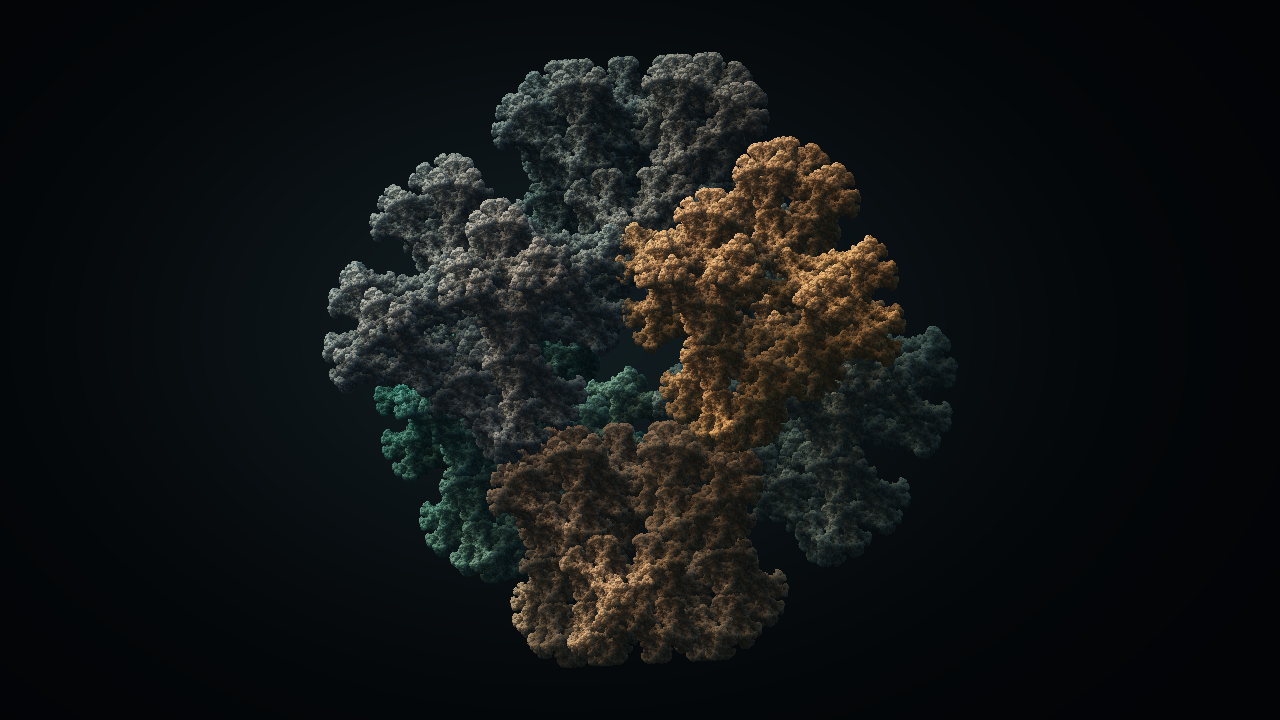
\includegraphics[width=.93\linewidth]{../site/assets/sixfold.png}
\caption{A finite rendering of the reference member, with two opposite lobes
coloured for orientation. The mathematical object is the compact attractor
defined in Section~\ref{sec:def}, not the shaded surface or a finite point cloud.
Image from the project visualisation archive.}
\label{fig:shape}
\end{figure}

\section{Exact definition of the family}\label{sec:def}
For $k\in\{0,\ldots,5\}$ set
\begin{equation}\label{eq:maps}
\begin{split}
\phi_k&=k\pi/3,\qquad \sigma_k=(-1)^k,\\
a_k&=(-\sin\phi_k,\cos\phi_k,0),\\
t_k&=(\cos\phi_k,\sin\phi_k,\sigma_k h),\\
G_k(x)&=rQ_kx+t_k,\qquad Q_k=R_{a_k}(\sigma_k\alpha).
\end{split}
\end{equation}
Here $R_a(\beta)$ is the right-handed rotation
\[
R_a(\beta)x=\cos\beta\,x+(1-\cos\beta)(a\cdot x)a+\sin\beta(a\times x).
\]
We use $u=\tan(\alpha/2)$, so that
$\cos\alpha=(1-u^2)/(1+u^2)$ and $\sin\alpha=2u/(1+u^2)$.
For a word $w=w_1\cdots w_n$, write
$G_w=G_{w_1}\circ\cdots\circ G_{w_n}$: the first digit is the outermost map.
For $0<r<1$, the attractor is the unique nonempty compact set
\begin{equation}\label{eq:attractor}
K=\bigcup_{k=0}^5G_k(K).
\end{equation}

The contact words are
\[
W=01153513,\qquad W'=10024204.
\]
Write $G_W(x)=M_Wx+c_W$ and define
\begin{equation}\label{eq:contact}
p(r,u,h)=(I-M_W)^{-1}c_W,\qquad
F(r,u,h)=\begin{pmatrix}-p_x/2+\sqrt3p_y/2\\p_z\end{pmatrix}.
\end{equation}
The inverse exists because $\|M_W\|=r^8<1$.

\begin{definition}[Root selection]\label{def:root}
Let $I_h=[0.7070,0.7072]$ and let the following terminating decimals denote
\emph{rational centres}, not exact fractal parameters:
\begin{align*}
r_c&=0.476178386161547669525964558546828831852499529292214482,\\
u_c&=0.2676240856235760042362757034639861560899940849527665828.
\end{align*}
For each $h\in I_h$, choose the unique zero $(r(h),u(h))$ of $F(\cdot,\cdot,h)$
in $|r-r_c|\le0.001$, $|u-u_c|\le0.001$. The resulting attractor is $K(h)$.
The \emph{reference member} is $K(h_0)$, where $h_0=1/\sqrt2$.
\end{definition}

Existence and uniqueness in this definition are the first certified claim.
The chosen branch has the sharper enclosure
\begin{equation}\label{eq:box}
|r-r_c|\le0.000007,\qquad |u-u_c|\le0.000060,
\qquad 0.476171<r<0.476186.
\end{equation}
At $h_0$, the root is isolated within $10^{-25}$ of each displayed centre;
$\alpha\approx29.965238257844163^\circ$. The unusually long centres make the
reference isolation reproducible; rounding them and declaring the resulting
maps exact would generally destroy the prescribed contact.

\subsection{Symmetries and the common periodic point}
Let
\[
S=\begin{pmatrix}1/2&\sqrt3/2&0\\\sqrt3/2&-1/2&0\\0&0&-1\end{pmatrix}.
\]
This is the half-turn about the horizontal axis at azimuth $\pi/6$.
Direct substitution in~\eqref{eq:maps} gives
$SG_kS^{-1}=G_{1-k\pmod6}$ and hence $G_{W'}=SG_WS^{-1}$.
Equation~\eqref{eq:contact} says $Sp=p$, so both word maps fix $p$.
The periodic addresses $W^\infty$ and $(W')^\infty$ therefore yield the same
point, with
\[
p\in G_0(K)\cap G_1(K).
\]
At the reference, $p\approx(1.15976670328374,0.66959161833803,0)$.

Let $T$ rotate by $\pi/3$ about the vertical axis and reverse $z$.
Then $TG_kT^{-1}=G_{k+1\pmod6}$, so $T(K)=K$. In particular $T^3=-I$,
$K=-K$, $Q_{k+3}=Q_k$, and $t_{k+3}=-t_k$.
These are exact symmetries throughout the family. At $h_0$ the six translations
are vertices of a regular octahedron; this fact does not make the rotated
attractor the classical Sierpi\'nski octahedron.

\subsection{Parameter certification}
Write $x=(r,u)$ and fix a rational matrix $C$ approximating the inverse of
$D_xF$ at the reference. The verifier encloses
\[
T_h(x)=x-CF(x,h),\qquad D_xT_h=I-CD_xF.
\]
On each certified rectangle it proves that $T_h$ maps the rectangle strictly
into itself and has sup-norm derivative less than one, uniformly in the
specified height interval. Banach's theorem gives a unique fixed point.
The derivative bound also makes $CD_xF$ invertible, and hence $C$ invertible,
so fixed points are exactly zeros of $F$.

The tight reference certificate has derivative bound below
$3.56\times10^{-23}$ and inclusion margins exceeding $9.99\times10^{-26}$.
The sharper family rectangle has derivative bound below $0.014467$, with
coordinate margins greater than $5.79\times10^{-7}$ and $1.45\times10^{-6}$.
A separate enclosure supplies uniqueness on the larger rectangle in
Definition~\ref{def:root}. The affine dependence of $F$ on $h$ for fixed
$(r,u)$ is preconditioned before interval evaluation to retain cancellations.
The uniform contraction implies continuous dependence on $h$; the usual
implicit-function argument applies locally since $D_xF$ is invertible.

\section{Connectedness, intersections and uniform dimension bounds}
\begin{theorem}\label{thm:geometry}
For every $h\in I_h$, $K(h)$ is connected and path connected. Its first-level
intersection graph is the octahedral graph: each $G_k(K)$ meets the four
nonopposite pieces, and is disjoint from $G_{k+3}(K)$. Moreover,
\begin{equation}\label{eq:uniformdim}
2.1970<\dimH K(h)<2.4150.
\end{equation}
Consequently $K(h)$ has full affine span, zero three-dimensional Lebesgue
measure, and empty interior.
\end{theorem}

\begin{proof}[Argument and finite certificates]
The six $T$-images of the periodic contact give the adjacent cycle in the
intersection graph. Hata's criterion gives connectedness; a connected
self-similar attractor is also locally connected and path connected
\cite{hata}. For the remaining nonopposite contacts use reflection
\[
V=\begin{pmatrix}-1/2&\sqrt3/2&0\\\sqrt3/2&1/2&0\\0&0&1\end{pmatrix},
\qquad n=(\sqrt3/2,-1/2,0).
\]
It exchanges pieces $0$ and $2$ and fixes $n\cdot x=0$.
If $p_k$ is the fixed point of $G_k$, interval arithmetic gives
$n\cdot p_0>1.6282$ and
$n\cdot G_0G_3G_3G_1(p_3)<-0.0136$ on the whole family.
Both points belong to the connected set $G_0(K)$, which therefore meets the
reflection plane and hence $G_2(K)$. Symmetry covers all such pairs.

For enclosures and dimension bounds, the archive contains all $6^8=1,679,616$
depth-eight centres on the grid $Q=2^{29}$. The integer recurrence has the form
$z\mapsto\lfloor A_kz/Q\rfloor+b_k$, coordinatewise, with stored integer
$A_k,b_k$. Error propagation bounds the difference between these grid centres
and the exact word centres $G_w(0)$ by $10^{-6}$ at the reference and
$0.00055$ uniformly on the family. Starting with an invariant ball of radius
$2.5$, the same calculation improves the enclosure to
\begin{equation}\label{eq:tail}
K\subset B(0,2.14),\qquad
G_w(K)\subset B(G_w(0),2.14r^{|w|}).
\end{equation}
Thus the opposite first-level pieces have gap at least
$2\sqrt{1+0.7070^2}-2(0.476186)(2.14)>0.4112$.

The certificate selects $M=461,042$ depth-eight words whose entire enclosing
balls are pairwise disjoint, uniformly in $h$. These word maps form a strongly
separated subsystem with attractor inside $K$, of dimension
$\log M/[8\log(1/r)]$. The unrestricted covering by $6^n$ cylinders gives
$\dimH K\le\log6/\log(1/r)$. The parameter interval~\eqref{eq:box} gives
\eqref{eq:uniformdim}. The strict lower bound above two also proves that $K$
is contained in no affine plane. The remaining consequences are immediate.
\end{proof}

The packing separation is checked with integers, not a floating-point nearest
neighbour decision. If $\rho=2.14r^8+\varepsilon$, the verifier chooses an
integer $L\ge Q\rho$ and tests against $D=2L+1$. For the family,
\begin{gather*}
L=3,332,642,\qquad D=6,665,285,\\
\min\|z_i-z_j\|^2=44,437,886,217,755>D^2=44,426,024,131,225.
\end{gather*}
The exact spatial-cell test checks the possible close pairs in the 27
neighbouring cells; more distant cells cannot violate separation. A separate
reference packing contains $464,873$ words. Its weaker lower bound is
superseded by the exact reference dimension below.
The intersection graph specifies which pairs meet, but not the cardinality,
dimension or topology of any intersection set.

\section{Separation failure and full Assouad dimension}\label{sec:assouad}
The open set condition (OSC) asks for a nonempty open set $O$ with
$G_k(O)\subset O$ and pairwise disjoint $G_k(O)$. We use the weak separation
property (WSP) in the usual relative-map form: the identity is not an
accumulation point of the nonidentity maps $G_v^{-1}G_w$.
The Assouad dimension controls the worst local covering rate, uniformly over
centres and over pairs of scales, rather than just the total small-scale size.

\begin{theorem}\label{thm:assouad}
For every $h\in I_h$, the six-map system fails OSC and WSP and
$\dimA K(h)=3$. No finite IFS of contracting similarities with the same
attractor can satisfy WSP, or consequently OSC.
\end{theorem}

\begin{proof}
Put $q=r^8$ and write the contact maps as
\[
G_W(x)=p+qA(x-p),\qquad G_{W'}(x)=p+qB(x-p),\qquad B=SAS^{-1}.
\]
If OSC held, a ball $B(x,\epsilon)\subset O$ would have $2^m$ disjoint images
under length-$m$ words in these two blocks. Every image has radius
$q^m\epsilon$ and lies within $B(p,q^m(\|x-p\|+\epsilon))$.
Volume comparison would bound $2^m$ by
$[(\|x-p\|+\epsilon)/\epsilon]^3$ for all $m$, a contradiction.

We next verify the rotation hypotheses. Both the local pair $Q_0,Q_1$ and
the block pair $A,B$ have distinct rotation axes and nonzero principal angles
less than $60^\circ$. The finite certificates are:
\begin{center}\small
\begin{tabular}{lll}\toprule
Pair & Trace interval for either member & Nonzero component of axial cross product\\\midrule
$Q_0,Q_1$ & $(2.7324,2.7329)$ & $z\in(-0.8647,-0.8637)$\\
$A,B$ & $(2.7105,2.7252)$ & $x\in(0.2024,0.2148)$\\\bottomrule
\end{tabular}
\end{center}
Here the axial vector of $R$ is
$(R_{32}-R_{23},R_{13}-R_{31},R_{21}-R_{12})$.
The classification of closed subgroups of $\SO(3)$ \cite[Section 3]{olive}
implies that each pair generates a dense subgroup: proper axis-preserving
groups cannot contain such rotations about distinct axes, and the remaining
proper finite polyhedral groups have no nontrivial rotation of angle less
than $72^\circ$. Positive products have the same closure as the group,
since inverse powers lie in the compact closure of positive powers.

To prove WSP failure we need many \emph{equal-length} block products.
The conjugate rotations $A,B$ have the same order. If it is infinite,
$A^{m-j}B^j$ for $0\le j\le m$ are distinct: equality would equate nonidentity
powers about different axes. If their common order is finite, say $N$,
positive words represent the infinite group they generate. Infinitely many
distinct elements have representative lengths in one residue class modulo
$N$. Any finite selection can be padded with powers of $A^N$ to a common
length. Thus equal-length product sets have unbounded cardinalities.
Compactness supplies distinct, arbitrarily close products $C,D$ of equal
length. The corresponding relative maps are
\[
x\longmapsto p+C^{-1}D(x-p),
\]
which are nonidentity maps tending to the identity. This is WSP failure.

The full affine span, dense positive rotation products and WSP failure meet
the hypotheses of Garc\'ia's Corollary 1.6(1) \cite{garcia}, yielding
$\dimA K=3$. Fraser et al.'s Theorem 1.4 \cite{fhor} gives
$\dimA K=\dimH K$ for a full-span self-similar set with a WSP presentation.
The strict gap in~\eqref{eq:uniformdim} therefore rules out every such
alternative presentation of $K$.
\end{proof}

The last conclusion concerns finite systems of contracting similarities.
It does not classify affine, nonlinear or graph-directed descriptions, nor
does it assert that a set of Assouad dimension three contains a solid region.

\section{Exact Hausdorff dimensions at two members}\label{sec:exact}
\begin{theorem}\label{thm:exact}
At $h_0=1/\sqrt2$, and at the certified family member with $u=19/71$, distinct finite
words define distinct affine maps and
\[
\dimH K=\frac{\log6}{\log(1/r)}.
\]
The two dimensions have disjoint certified enclosures, with approximate values
\begin{align*}
\dimH K(h_0)&=2.414891458627539380224930\ldots,\\
\dimH K(h_1)&=2.414905234586818002788584\ldots,
\end{align*}
where $h_1\approx0.70714070075078310161$. These two members are not bi-Lipschitz
equivalent.
\end{theorem}

The proof has three parts: algebraic parameter certification, distinction of
all finite word maps, and application of Hochman's algebraic theorem
\cite[Corollary 1.7]{hochman}. This last theorem applies to an algebraic,
linearly irreducible similarity system without exact overlaps. The dense
rotation group in Section~\ref{sec:assouad} supplies irreducibility. The
similarity dimension is below three.

\subsection{From three rotation letters to six affine maps}\label{sec:signs}
Since $Q_{k+3}=Q_k$ and $t_{k+3}=-t_k$, it suffices first to distinguish
equal-length products of the three rotation letters indexed by residues
modulo three. All translations have length $L=\sqrt{1+h^2}$.
Equal affine maps must have equal word lengths, because their contraction
ratios agree. If their rotation products determine the residue sequences,
the first remaining difference is a translation sign at some index $j$,
counting from zero. Its contribution has length $2Lr^j$, whereas the sum of
all later differences has length at most
\[
\frac{2Lr^{j+1}}{1-r}<2Lr^j,
\]
using $r<1/2$. Cancellation is impossible. A shared periodic fixed point is
therefore compatible with the absence of equal finite word maps.

\subsection{The rational-tilt member: a finite-field argument}
We present the shorter example first. In coordinates $(x,\sqrt3y,z)$, the
rotations have entries in $\mathbb Q(u)$. Put $v=(1,1,0)$ and
$D=2(1+u^2)$. Writing the translation of $G_W$ as $c_0+hc_1$ in these
coordinates, define polynomial columns
\[
a=D^8(v-r^8Q_Wv),\qquad b=2D^8c_0,\qquad d=2D^8c_1.
\]
The contact equation is $2\lambda a=b+hd$. At $u=19/71$ its determinant
$a\cdot(b\times d)=0$, after removing fixed factors, is a degree-22
polynomial in $r$. The verifier isolates a root
$r\approx0.47618040162277722027$. An invertible two-row subsystem recovers
$h$ by Cramer's rule, and the determinant enforces the third row.
Exact rational bounds place $(r,u,h)$ on the branch of
Definition~\ref{def:root}. In particular $r,h$ are algebraic.

Multiply the three scaled-coordinate rotations by $71^2+19^2=5402$.
Their reductions modulo $37$ are
\[
\begin{pmatrix}18&0&34\\0&0&0\\3&0&18\end{pmatrix},\quad
\begin{pmatrix}23&23&20\\32&32&23\\17&17&18\end{pmatrix},\quad
\begin{pmatrix}23&14&20\\5&32&14\\17&20&18\end{pmatrix}.
\]
Each has rank one. Their image lines are distinct, spanned by
$(1,0,31)$, $(1,3,12)$ and $(1,34,12)$, and all nine ordered two-letter
products are nonzero. Consequently every product is nonzero with the image
line of its first letter. Equal-length real rotation products would be equal
after multiplication by the common denominator and reduction modulo $37$.
Their first letters must agree. Cancel that invertible letter over the reals
and repeat. This proves the required rotation-word distinction at every length.
Section~\ref{sec:signs} and Hochman's theorem give the second dimension.

\subsection{The reference member: elimination and a complex conjugate}
For $h_0^2=1/2$ the same columns give the polynomial equations
\begin{equation}\label{eq:elimination}
a\cdot(b\times d)=0,\qquad
2(a\times b)_y^2-(a\times d)_y^2=0.
\end{equation}
Removing integer content and the factors $(1+u^2)^{17}$ and
$(1+u^2)^{16}$, respectively, leaves bidegrees $(22,14)$ and $(30,32)$ in
$(r,u)$. Their resultant in $r$ has degree $1094$, with factor degrees and
multiplicities
\[
(1,46),\quad(2,126),\quad(182,2),\quad(432,1).
\]
Interval evaluation in the reference box excludes the first three factors.
The stored degree-432 polynomial $f$ is checked by reconstructing the
resultant and multiplying its factors. Its irreducibility over $\mathbb Q$
is certified by squarefree, degree-preserving reductions at $7,13,37,43$:
the possible factor-degree subset sums common to all four are only $0,432$.
Thus $f$ is the minimal polynomial of the reference tilt $u$.
The first equation in~\eqref{eq:elimination} then proves $r$ algebraic:
its nonzero coefficients in $u$ have degree at most $14$, so cannot vanish
at a root of degree $432$.

An exact Gaussian-integer Rouch\'e check isolates a root $\zeta$ of $f$ in
the disk of radius $10^{-10}$ about
\[
-0.028547283375+1.138685386817\,i.
\]
After substituting the centre plus $10^{-10}w$, the linear term exceeds the
sum of all other terms by a factor greater than $100$ on $|w|=1$.
It follows that there is exactly one root in this disk. Irreducibility makes
it an algebraic conjugate of the real reference $u$.

Here is the all-length step. Regard the three oriented axes as spaced by
$120^\circ$, with each generator having positive angle $\alpha$.
Any identity between their real rotation words transfers to $\zeta$, because
the scaled-coordinate matrices are rational over $\mathbb Q(u)$ and their
denominators do not vanish there. Use the projective lifts
\[
L_a(z)=I-iz(a\cdot\boldsymbol\sigma),
\]
where $\boldsymbol\sigma$ are the Pauli matrices. Conjugation on traceless
matrices implements the complexified Rodrigues rotation; this identity is
checked symbolically. Equal rotation words thus give equal projective
transformations on $\mathbb{CP}^1$.

On its unit-sphere model, the eigenlines are $+a,-a$. The ratio of minus to
plus eigen-coordinates of a point at spherical angle $\delta$ from $+a$ has
modulus $\tan(\delta/2)$. Applying $L_a(\zeta)$ multiplies this modulus by
\[
\left|\frac{1+i\zeta}{1-i\zeta}\right|<0.067
< (2-\sqrt3)^2=\tan^2(15^\circ).
\]
Take the three disjoint closed caps of radius $30^\circ$ about the positive
axes. Each point in their union is at least $30^\circ$ from every negative
axis. Therefore each generator sends the whole union into the interior of
its own cap. The image identifies the first letter of a nonempty word.
Cancellation and induction distinguish all equal-length words.
Section~\ref{sec:signs} now proves absence of exact overlaps in the six-map
system. Hochman's theorem yields the reference dimension.

The reference dimension is enclosed by
\[
2.414891458627539380224930\ \mathbin{\pm}\ 9.77\times10^{-25}.
\]
The second enclosure has width less than
$6\times10^{-32}$ and is disjoint from the first. Since Hausdorff dimension
is invariant under bi-Lipschitz maps, the final assertion of
Theorem~\ref{thm:exact} follows. No exact dimension formula for every $h\in I_h$
is asserted here.

\section{Passages and loops in the full attractor}\label{sec:loops}
Throughout this section $h\in I_h$. Homology means integral \emph{singular}
homology. A loop is a continuous map from the circle and need not be an
embedded polygon or a smooth curve. We use winding and linking homomorphisms
on the complement of a line or a polygonal wire; these are defined for
arbitrary continuous loops and depend only on their homology classes.

\subsection{A central passage and its winding loop}
\begin{proposition}\label{prop:central}
The closed vertical cylinder of radius $0.0122$ is disjoint from $K$.
There is a loop $\gamma$ in $K$ with winding number one about its axis.
\end{proposition}
\begin{proof}
In the depth-eight grid calculation restricted to $G_0(K)$, the minimum
integer $x$-coordinate is $3,049,454$ and the minimum squared horizontal
radius is $97,951,509,407,090$. Put
$\epsilon=0.00055+2.14(0.476186)^8$. Every attractor point in this piece is
within $\epsilon$ of an appropriate grid centre. Since each centre has
positive $x$, its distance to the half-plane
$H=\{(x,0,z):x\le0\}$ equals its horizontal radius. The exact squared-distance
test proves that its distance to $H$, after subtracting $\epsilon$, exceeds
$0.0122$. Symmetry under $T$ proves cylinder avoidance for all pieces.

The adjacent contact points $T^{-1}p,p$ belong to $G_0(K)$ and lie at
azimuths $-\pi/6,\pi/6$. Their positive radial coordinates are certified by
the contact enclosures. Join them by a path in $G_0(K)$, using path
connectedness. Avoidance of $H$ permits a continuous principal argument
along the path, with total change $\pi/3$. Concatenating its six images
under $T^j$, $0\le j<6$, yields a closed loop with total argument change
$2\pi$. Projection to the circle gives a homomorphism detecting its
nonzero homology class in the full $K$.
\end{proof}

\subsection{Two smaller passages and independent classes}
Define parallel lines, oriented by $d=(-1,0,1)/\sqrt2$, by
\begin{equation}\label{eq:axes}
\ell_\pm=\{(x,0,z):x+z=\pm(1+h)\}.
\end{equation}
Let $\gamma_A=G_0\gamma$ and $\gamma_B=G_3\gamma$.
\begin{proposition}\label{prop:two}
For each sign, $0.105<\dist(K,\ell_\pm)<0.118$. With consistent orientations,
the winding numbers of $\gamma_A,\gamma_B$ about these lines form the identity
matrix. Thus $[\gamma_A],[\gamma_B]$ are linearly independent in $H_1(K;\Z)$.
\end{proposition}
\begin{proof}[Certificate and winding argument]
For sign $s=\pm1$, perpendicular coordinates are
$(X/\sqrt2,Y)$, with $X=x+z-s(1+h)$ and $Y=y$.
The verifier evaluates
\[
(i+k-sQ(1+\widehat h))^2+2j^2
\]
at all grid centres $(i,j,k)$, where
$\widehat h=\lfloor0.7071Q\rfloor/Q$. This is twice the squared physical
line distance after division by $Q^2$. The grid, height and cylinder-tail
allowances give a total distance error less than $0.00631$.
The resulting interval is contained in $(0.105,0.118)$ for both lines.

For each of the six subpieces of the relevant child, the verifier also
certifies a half-plane inequality
\[
\frac{aX+bY}{\sqrt{2a^2+b^2}}>0.06,
\quad (a,b)\in\{(1,0),(-1,2),(1,2),(-1,0),(1,-2),(-1,-2)\},
\]
with the listed normals assigned to the six successive subpieces.
Each projected path segment may therefore be homotoped to its endpoint
chord without crossing the projected origin. The resulting contact hexagon
has winding one: the map on the contact plane for the upper child has
matrix $\operatorname{diag}(r(\cos\alpha-\sin\alpha)/\sqrt2,r)$, with
positive determinant. Symmetry supplies the lower child.
Each child is contained in a ball of radius $2.14r$ clearing the other line
by more than $1.39$, so the two cross-windings vanish. The two winding
homomorphisms read off the coefficients in any relation between the classes.
\end{proof}

\begin{figure}[tb]
\centering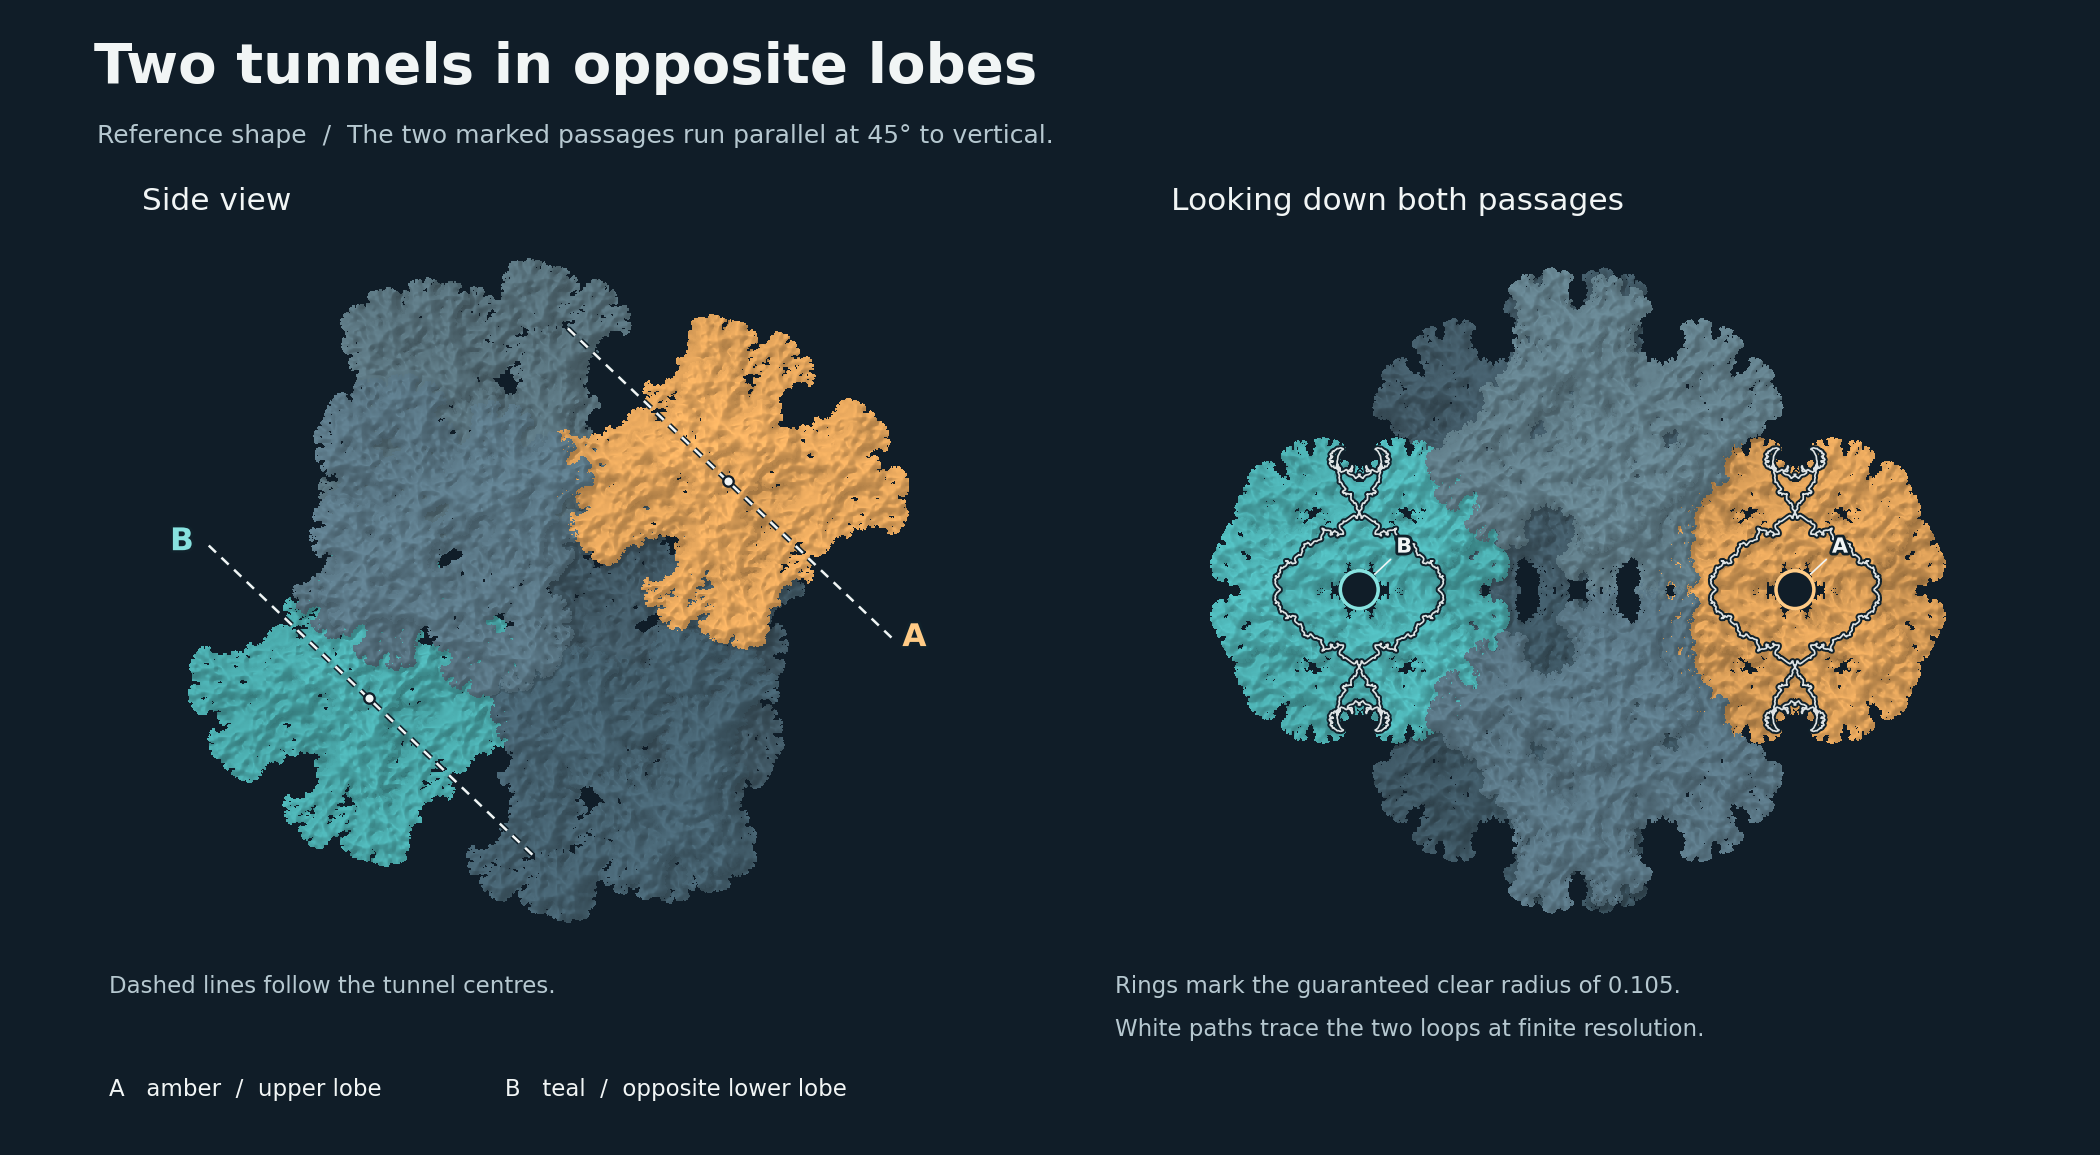
\includegraphics[width=\linewidth]{../research/fractal_research_09/opposite_tunnels.png}
\caption{The two clear lines~\eqref{eq:axes}, with the upper and opposite lower
lobes marked A and B. The rings show a guaranteed clear radius $0.105$;
the drawn paths are finite approximations to the loops used in the argument.
The line directions differ from the original inherited tilted axes discussed
in Section~\ref{sec:bore}.}
\label{fig:two}
\end{figure}

\subsection{Detecting wires at every scale}
The essential question for a repeated loop is whether a neighbouring piece
could fill it in the full attractor. The following construction supplies
detecting curves that avoid \emph{all} pieces.

\begin{theorem}\label{thm:homology}
For every $h\in I_h$ there are countably many linearly independent classes
in $H_1(K(h);\Z)$ represented by loops shrinking to the fixed point $p_*$
of $G_0$. There is a surjective homomorphism
\begin{equation}\label{eq:product}
H_1(K(h);\Z)\longrightarrow\prod_{m\ge0}\Z.
\end{equation}
In particular this homology group is uncountable. At each of the six
symmetry-related fixed points there are arbitrarily small loops that remain
noncontractible in the entire attractor.
\end{theorem}

\begin{proof}
The point $p_*=(I-rQ_0)^{-1}t_0$ is distinct from the periodic contact $p$;
at the reference it is approximately $(1.88117,0,0.44205)$. Set
\[
t=(1,0,h),\quad e=(1,0,1)/\sqrt2,\quad d=(-1,0,1)/\sqrt2,
\quad a=1.03,
\]
and let $D$ be the boundary of the rectangle
\[
\{t+ve+wd:0\le v\le a,\ |w|\le a\}.
\]
Its edge $v=0$ lies on $\ell_+$, which is clear of $K$.
The other three edges are outside $B(t,2.14r)$, since $a>2.14r$.
All sibling enclosing balls lie strictly in $e\cdot(x-t)<0$, so the full
wire misses $K$. Orient $D$ so that its edge on $\ell_+$ follows $d$.
Then $\lk(\gamma_A,D)=1$. Indeed, compactify the line in $S^3$ and replace
its exterior arc by the three remaining rectangle edges. Both arcs lie
outside the child ball and are homotopic relative to endpoints there,
because the exterior of a ball in $S^3$ is simply connected.

The following four strict bounds are interval-certified over the whole family:
\begin{equation}\label{eq:wires}
\begin{split}
\dist\left(p_*,\bigcup_{k\ne0}G_k(K)\right)&>0.96,\\
G_0(D)&\subset B(p_*,0.95),\\
\dist(p_*,D)&>0.19,\\
G_0^4(G_0(K))&\subset B(p_*,0.11).
\end{split}
\end{equation}
The second bound follows from the four rectangle corners and convexity of
the ball. As $G_0$ fixes $p_*$ and contracts, all its later wire images
remain within $B(p_*,0.95)$. Inductively, $G_0^j(D)$ avoids $G_0(K)$ by
injectivity if $G_0^{j-1}(D)$ avoids $K$, and it avoids the siblings by
the first bound. Thus every wire image misses the entire attractor.

For $n,m\ge0$ put
\[
\gamma_n=G_0^{4n}(\gamma_A),\qquad D_m=G_0^{4m}(D).
\]
Similarity invariance gives $\lk(\gamma_m,D_m)=1$. For $n>m$, apply
$G_0^{-4m}$ and use~\eqref{eq:wires}: the smaller loop lies in
$B(p_*,0.11)$, disjoint from $D$. Hence
\begin{equation}\label{eq:triangular}
\lk(\gamma_n,D_m)=
\begin{cases}1,&n=m,\\0,&n>m.\end{cases}
\end{equation}
No assertion is made about entries with $n<m$. Pairing a finite relation
against the wire at its smallest index reads off that coefficient.
Induction gives linear independence.

For the stronger assertion, base $\gamma_A$ at $p_*$ by an out-and-back path
inside $G_0(K)$ and call the resulting loop $\beta_0$.
Set $\beta_n=G_0^{4n}\beta_0$. The connecting paths add no linking number.
For any target integer sequence $(b_m)_{m\ge0}$, recursively choose
\[
c_m=b_m-\sum_{n<m}c_n\lk(\beta_n,D_m).
\]
Concatenate $\beta_m^{c_m}$ on successive time intervals of lengths
$2^{-m-1}$ and end at $p_*$. Each $c_m$ is finite, although the sequence
may be unbounded. The diameters of the based loops tend to zero, so the
infinite concatenation is continuous at its endpoint.
For any fixed $m$, the entire tail after stage $m$ lies in
$B(p_*,0.11r^{4m})$, disjoint from $D_m$ by~\eqref{eq:wires}.
That tail is null-homologous in the wire complement. The resulting loop
therefore has linking record exactly $(b_m)$, proving surjectivity.
The product is uncountable. Finally, symmetry transports the shrinking
essential loops to the other five fixed points.
\end{proof}

This is a quotient statement, not an identification of $H_1(K;\Z)$ with
the product. It does not classify the fundamental group or establish a
homeomorphism with the Hawaiian earring. Infinite concatenations of shrinking
loops are classical \cite[Example 1.25]{hatcher}; the geometry in
\eqref{eq:wires} is what validates their use in this overlapping spatial set.

\subsection{The original tilted bore: obstruction at positive radius}\label{sec:bore}
The original upper child's inherited central axis is the line through
$t=(1,0,h)$ with unit direction $v=(\sin\alpha,0,\cos\alpha)$.
For a point $P=(x,y,z)$ define inward travel and perpendicular distance by
\[
T(P)=-v\cdot(P-t),\qquad
D(P)^2=[\cos\alpha(x-1)-\sin\alpha(z-h)]^2+y^2.
\]
For bore radius $0.0058$, the first intrusion is
$\min\{T(P):P\in K,\ D(P)\le0.0058\}$.
The certificate encloses it in $[1.325115,1.325120]$ at the reference and
in $[1.320,1.330]$ uniformly on the family. Lobes 1 and 5 intrude in the
upper bore; central inversion gives lobes 4 and 2 for the lower bore.
At the reference, the first occupied axis cross-section is near
$(0.33814,0,-0.44088)$.

An actual point with address $1404022400020420424\,0^\infty$ is inside the
reference bore, near $(0.340917,0.004592,-0.442484)$. Its mirror supplies
the other intrusion. This proves nonemptiness of the compact minimisation
set. The lower travel bound follows by discarding word balls from
\eqref{eq:tail} that lie outside the bore or beyond the proposed threshold;
all remaining reference branches close by depth 16. A separate addressed
witness supplies the uniform upper bound.

\begin{figure}[tb]
\centering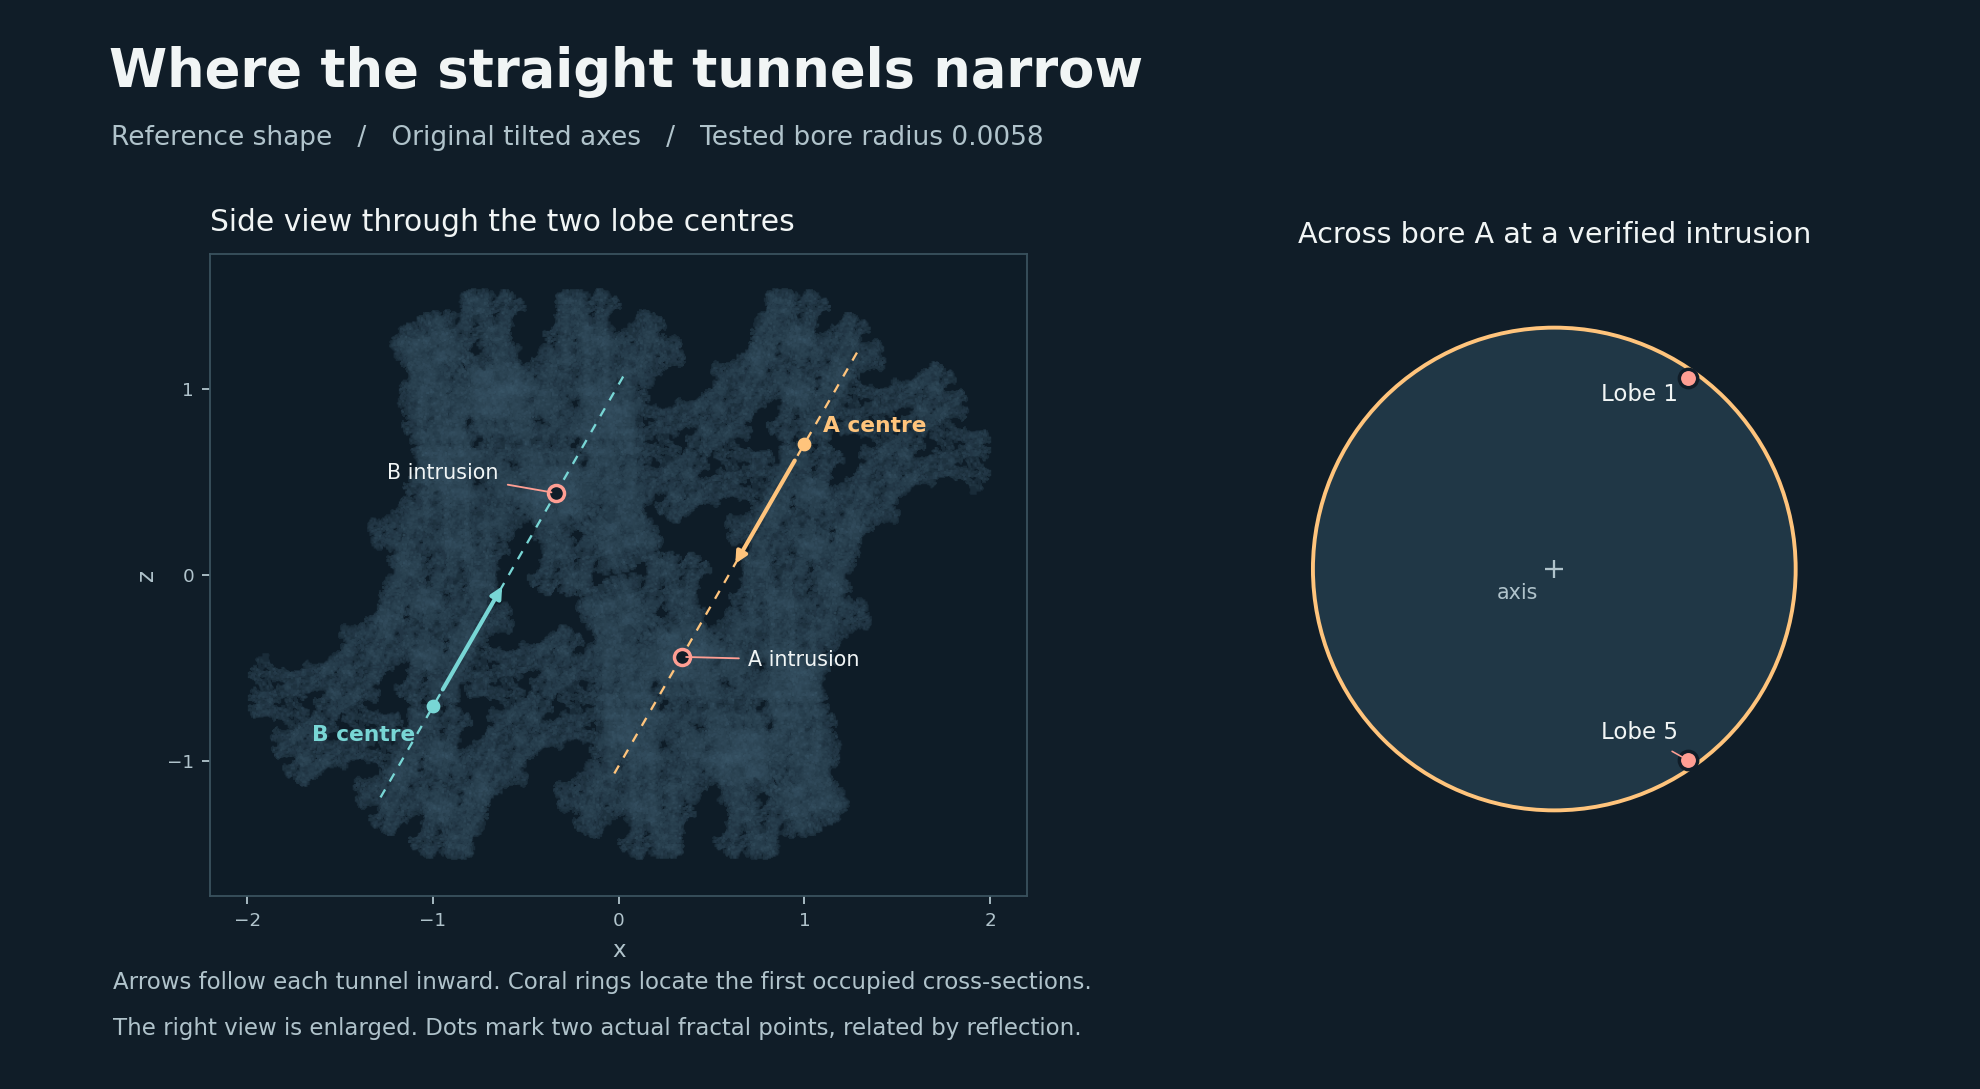
\includegraphics[width=\linewidth]{../research/fractal_research_10_topology/straight_axis_locator.png}
\caption{Obstruction of the inherited tilted bores at radius $0.0058$.
The enlarged cross-section marks actual addressed fractal points in lobes
1 and 5. Occupation of a positive-radius bore does not establish an exact
intersection with its centreline.}
\label{fig:bore}
\end{figure}

Whether the zero-width inherited axis meets $K$ remains open. Extremely close
addressed points and surviving branches of a finite search do not prove an
exact hit. The clear lines~\eqref{eq:axes} and Theorem~\ref{thm:homology} do
not depend on resolving this question. Here a ``tunnel'' denotes a certified
passage in the complement accompanied by a detected loop; it does not assume
a smooth wall or a solid body with a well-defined genus.

\section{Related constructions and the scope of originality}\label{sec:originality}
The comparison uses the repository's 17 November 2026 search, with original
sources rechecked and supplemented on 18 November 2026. It covers the
Sierpi\'nski octahedron, polyhedral gaskets, rotated and kaleidoscopic IFSs,
periodic contacts, connected systems without separation, and mathematical-art
sources. This is a bounded literature comparison, not an exhaustive priority
search or a classification of equivalent IFS presentations.

\subsection{Spatial and visual relatives}
The regular Sierpi\'nski octahedron studied by Kunnen and Schlicker
\cite{kunnen} is a close geometric comparator. With vertex set $V$ its maps
are $f_v(x)=(x+v)/2$. All six first-level pieces contain the centre, since
$-v$ belongs to the attractor and $f_v(-v)=0$. In contrast, Sixfold's central
axis is clear. The classical dimension $\log6/\log2=2.58496\ldots$ differs
from every dimension allowed by~\eqref{eq:uniformdim}. Thus these sets are
not bi-Lipschitz equivalent. This does not decide homeomorphism.

Tsuiki's triangular-antiprismoid construction \cite{tsuiki} is another
six-vertex spatial fractal, with dimension two and square projections.
Fathauer, Kaczmarski and Duchnowski's fractal crystal \cite{fathauer}
supplies a mathematical-art precedent for recursive polyhedral structures
and an octahedral outline. Neither visual similarity nor a shared symmetry
group identifies an attractor. The standard Menger sponge, generated by
twenty one-third-scale cube similarities satisfying OSC, has dimension
$\log20/\log3=2.72683\ldots$. This also distinguishes metric geometry,
without resolving the topological comparison.

The Fragmentarium octahedral shader \cite{syntopia} is a particularly close
programmable precedent for rotated octahedral imagery. Its 2010-labelled
source credits Knighty's kaleidoscopic construction; we compare the immutable
July 2011 source version. On a linear branch of one fold iteration the
orthogonal matrix is $AP_iB$, where $A,B$ are common orthogonal matrices and
$P_i$ is a signed permutation. Relative branch matrices, also for inverse
branches, are therefore conjugate to signed permutations. If orientation
preserving, their traces belong to $\{-1,0,1,3\}$.

In Sixfold the oriented axes for $Q_0,Q_1$ have dot product $-1/2$.
Quaternion multiplication gives
\begin{equation}\label{eq:shader}
\tr(Q_0^{-1}Q_1)=4\left(\frac{1-u^2/2}{1+u^2}\right)^2-1
\in(2.23,2.24)
\end{equation}
on the certified interval. Relative traces are unchanged by a global
similarity and branch relabelling. This rules out identity of the literal
one-step branch systems at any settings of that shader. It does \emph{not}
rule out equality of attractors from other maps or from regrouped iterations.
Informal artworks and presets without recoverable maps remain unresolved
comparisons; they cannot responsibly be declared equivalent or distinct.

\subsection{Overlap and dimension precedents}
Tetenov, Kamalutdinov and Vaulin \cite{arc} constructed a spatial
self-similar Jordan arc failing OSC and WSP. Thus connectedness in three
dimensions without separation is not new. Their arc cannot be homeomorphic
to Sixfold, whose nonzero homology is detected above. Kamalutdinov and
Tetenov's six-map example on the line \cite{uniquecontact} also shows that
one-point intersection need not imply OSC.

Broomhead, Montaldi and Sidorov's golden gaskets \cite{golden} are a planar
overlapping family with holes and special computable parameters. Bandt and
Mekhontsev \cite{bandt} study connected planar carpets with irrational
rotations found by computer-assisted search. These precede the broad ideas
of rotated self-similarity, parameter families and computer-guided discovery.
Their planar sets cannot be bi-Lipschitz equivalent to a Sixfold member,
since~\eqref{eq:uniformdim} places its Hausdorff dimension above two.

B\'ar\'any and Verma's recent work on common fixed-point structure
\cite{baranyverma}, first posted in 2025 and published online in 2026,
is also directly relevant to the contact mechanism. It concerns dimension
and separation for systems on the real line with maps sharing fixed points.
In that setting maps about a common point commute and produce word-map
equalities. Our common point is shared by spatial block maps with different
rotation axes; at the two selected members we prove that no distinct finite
word maps coincide. The shared-fixed-point idea itself is therefore not a
novelty claim.

The Hausdorff--Assouad gap and the use of algebraicity to determine dimension
belong to the existing theory cited in Sections~\ref{sec:assouad}
and~\ref{sec:exact}. Likewise, the general shrinking-loop mechanism is
classical. The proposed contribution is verifying those mechanisms and
hypotheses for this explicit spatial contact family.

\subsection{What can reasonably be claimed}
Within the sources examined, we have not identified the family specified
by~\eqref{eq:maps}--\eqref{eq:contact} with its certified root branch and the
same package of dimension and linking results. The most defensible claim
is therefore:
\begin{quote}
We describe an explicitly specified periodic-contact family of spatial
self-similar sets and provide reproducible computer-assisted arguments for
its dimensional, separation and homological properties.
\end{quote}
This is a claim about the construction and the analysis presented here.
It is not a claim of being the first twisted octahedral fractal, the first
connected overlapping spatial fractal, or a new topological type. Two
certified different dimensions establish at least two bi-Lipschitz classes
within this family. Pairwise inequivalence of all its members, and historical
priority for the exact construction, remain unresolved.

\section{Open problems and review priorities}\label{sec:open}
\paragraph{Dimension across the parameter curve.}
Does $\dimH K(h)=\log6/\log(1/r(h))$ hold for every $h\in I_h$?
The two algebraic proofs do not settle this. Neither numerical dimension
estimation nor continuity of the parameter curve supplies the missing
separation argument. Determining how many members are bi-Lipschitz distinct
is a related but separate problem.

\paragraph{Topology and intersections.}
Determine the full first homology and fundamental groups, the topological
dimension, and the structure of first-level intersection sets. The product
quotient in~\eqref{eq:product} does not classify these groups. A comparison
with the Menger sponge as a topological space requires topological
invariants; the different Hausdorff dimensions alone cannot decide it.
The current proof locates shrinking essential loops at six special fixed
points, not at every point of $K$.

\paragraph{The exact inherited centreline.}
Decide whether the original tilted zero-radius axis intersects the full
attractor. The certified positive-radius obstruction settles the practical
bore question but leaves exact incidence open. More finite-depth near hits
without an all-depth argument would not resolve it.

\paragraph{Extent and bifurcations of the family.}
The interval $I_h$ is a certified domain, not a maximal existence interval.
Continuing the contact branch, locating changes in intersection structure,
and finding other contact words may lead to a broader collection of families.
The present certificate does not justify extrapolating beyond its interval.

\paragraph{Independent mathematical review.}
The first review should check the exact root-selection rule and interval
inclusion proof, the compact-group/equal-length argument for WSP failure,
the hypotheses and versions of the two dimension theorems, the algebraic
conjugate and finite-field word arguments, and the full-set wire avoidance
and infinite-concatenation step. These are review tasks for existing claims,
distinct from the open research problems above. An independent
implementation of selected certificates would reduce shared-code risk.

\paragraph{Originality and publication.}
Further comparison should target rotated polyhedral IFS source code and
older mathematical-art constructions with explicit maps, allowing for
alternative presentations. A suitable initial publication is a documented
construction with computer-assisted proofs. Any stronger assertion of
priority should wait for a broader expert literature assessment. Once the
technical note is reviewed and revised, its precise source, compiled paper
and supporting evidence should receive a new archived version.

\section{Reproducibility, contributions and disclosure}\label{sec:repro}
The archive contains parameter certificates, exact integer packing data,
symbolic and interval verifiers, research reports, and rendering source.
The implementation uses pinned dependencies with Python 3.12, including
\texttt{python-flint==0.9.0} for exact elimination and ball arithmetic.
From the repository root, the aggregate verification command is
\begin{quote}\small\ttfamily
uv run --isolated --python 3.12\newline
\hspace*{1em}--with-requirements requirements.txt python scripts/verify.py\newline
\hspace*{1em}--receipt .build/verification.json
\end{quote}
The displayed line breaks are typographical; run it as one command.
The runner uses temporary research copies, enables assertions, and records
the research-tree hash and separate outcomes. On 18 November 2026 all six
groups passed using Python 3.12.9 on Windows: handover integrity and uniform
certificates; reference exact-dimension premises; second-member premises;
central passage; two independent passages; tilted-bore and shrinking-loop
premises. The full receipt accompanies this draft as
\texttt{paper/verification.json}, including the SHA-256 of the run's complete
research tree. That identifier includes visual assets and is distinct from
the Zenodo ZIP checksum. The claim register separates finite outputs from
the deductions to which they contribute.

The author, credited as \textbf{okwhynot-wtf}, initiated and directed the
investigation, selected its aims and presentation, and evaluated the visual
results. OpenAI GPT models, through ChatGPT and Codex, provided substantial
assistance with construction searches, proposed proofs, verification and
rendering code, literature searches, and preparation of this manuscript.
AI-generated mathematical arguments are not treated as independent review.
Specific historical model versions are not asserted where the session record
does not establish them. The human author is responsible for decisions about
publication and for arranging review of the claims.

The project code and original parameter/certificate data are MIT licensed;
writing and images are CC BY 4.0. Third-party works retain their own terms
and are cited rather than incorporated as project-owned material. The films
are supplementary visual communication, not prerequisites for reproducing
the mathematical definition or proofs.

\appendix
\section{Evidence map and proof dependencies}\label{app:evidence}
All links below identify files at the archived evidence commit. The
historical reports describe successive states of the work: an earlier
``open'' statement may be superseded by a later report. For current scope,
use the statements of this draft together with the claim register.

\begin{longtable}{@{}p{.22\linewidth}p{.73\linewidth}@{}}
\toprule Claim & Archived source and finite component\\\midrule\endhead
Exact family & \repo{research/fractal_handover/fractal_research_04/RESEARCH_04.md}{Phase 04 report}; \repo{research/fractal_handover/fractal_research_04/verify_positive_contact.py}{contact verifier}. Root rectangles, interval Jacobian and symmetry identities.\\[5pt]
Uniform bounds & \repo{research/fractal_handover/fractal_research_05/RESEARCH_05.md}{Phase 05 report}; \repo{research/fractal_handover/fractal_research_05/verify_dimension.py}{dimension verifier}. Integer centres, error bounds, stored word subsets and exact separation tests.\\[5pt]
Pair contacts / OSC & \repo{research/fractal_handover/fractal_research_06/RESEARCH_06.md}{Phase 06 report}; \repo{research/fractal_handover/fractal_research_06/verify_obstruction.py}{obstruction verifier}. Reflection crossing and opposing-ball separation.\\[5pt]
WSP / Assouad & \repo{research/fractal_handover/fractal_research_07/RESEARCH_07.md}{Phase 07 report}. Rotation-angle and distinct-axis enclosures, with compact-group and theorem-application arguments.\\[5pt]
Two exact dimensions & \repo{research/fractal_research_08/RESEARCH_08.md}{Phase 08 report}; \repo{research/fractal_research_08/verify_reference.py}{reference verifier}; \repo{research/fractal_research_08/verify_member.py}{rational-tilt verifier}; \repo{research/fractal_research_08/reference_tilt_polynomial.json}{degree-432 coefficient data}.\\[5pt]
Central loop & \repo{research/fractal_research_08/verify_tunnel.py}{Central-passage verifier} and the Phase 08 winding argument.\\[5pt]
Two independent loops & \repo{research/fractal_research_09/RESEARCH_09.md}{Phase 09 report}; \repo{research/fractal_research_09/verify_tunnels.py}{passage verifier}; \repo{research/fractal_research_09/tunnel_certificate.json}{certificate}. Whole-set clearances and projected half-plane margins.\\[5pt]
Shrinking loops / bore & \repo{research/fractal_research_10_topology/RESEARCH_10.md}{Phase 10 report}; \repo{research/fractal_research_10_topology/verify.py}{topology verifier}; \repo{research/fractal_research_10_topology/certificate.json}{certificate}. Addressed points, exhaustive branch exclusions and four wire bounds.\\[5pt]
Prior-art comparison & \repo{research/fractal_research_11_prior_art/PRIOR_ART.md}{Original comparison report}; external sources below. Section~\ref{sec:originality} adds the B\'ar\'any--Verma comparison and corrects/checks bibliography metadata.\\\bottomrule
\end{longtable}

The main dependencies are: root isolation $\to$ periodic contacts $\to$
connectedness; packing and cylinder bounds $\to$ uniform dimension and
clearances; common contact plus rotation certificates $\to$ WSP failure
$\to$ Assouad dimension; algebraicity and word distinction $\to$ the two
exact Hausdorff dimensions; path connectedness plus clearances $\to$ winding
loops $\to$ full-set detecting wires $\to$ the homology quotient.
No argument uses a finite rendering as evidence of an exact contact,
nonintersection or homology class.

\begin{thebibliography}{99}
\bibitem{sixfold}
okwhynot-wtf.
\emph{Sixfold: research repository and visualisation archive}, version
\texttt{zenodo}, 18 November 2026.
\href{https://doi.org/10.5281/zenodo.24336419}{doi:10.5281/zenodo.24336419}.
Evidence commit \texttt{1c660bedf8cd3e52bad8e5d033535dcde6e06b6e}.

\bibitem{hutchinson}
J.~E. Hutchinson.
Fractals and self-similarity.
\emph{Indiana University Mathematics Journal} \textbf{30}(5) (1981), 713--747.
\href{https://doi.org/10.1512/iumj.1981.30.30055}{doi:10.1512/iumj.1981.30.30055}.

\bibitem{hata}
M. Hata.
On the structure of self-similar sets.
\emph{Japan Journal of Applied Mathematics} \textbf{2}(2) (1985), 381--414.
\href{https://doi.org/10.1007/BF03167083}{doi:10.1007/BF03167083}.

\bibitem{badgervellis}
M. Badger and V. Vellis.
H\"older parameterization of iterated function systems and a self-affine phenomenon.
\href{https://arxiv.org/abs/1910.08850v3}{arXiv:1910.08850v3}, 2020
(first posted 2019). Theorem 1.1, with a direct proof of path connectedness
without a separation assumption.

\bibitem{hochman}
M. Hochman.
On self-similar sets with overlaps and inverse theorems for entropy in $\R^d$.
\href{https://arxiv.org/abs/1503.09043v2}{arXiv:1503.09043v2}, 2017
(first posted 2015). Corollary 1.7 in the cited version.

\bibitem{garcia}
I. Garc\'ia.
Assouad dimension and local structure of self-similar sets with overlaps
in $\R^d$.
\href{https://arxiv.org/abs/1909.03148v2}{arXiv:1909.03148v2}, 2020
(first posted 2019). Corollary 1.6(1) in the cited version.

\bibitem{fhor}
J.~M. Fraser, A.~M. Henderson, E.~J. Olson and J.~C. Robinson.
On the Assouad dimension of self-similar sets with overlaps.
\emph{Advances in Mathematics} \textbf{273} (2015), 188--214.
\href{https://doi.org/10.1016/j.aim.2014.12.026}{doi:10.1016/j.aim.2014.12.026}.
Theorem 1.4 also in \href{https://arxiv.org/abs/1404.1016v2}{arXiv:1404.1016v2}.

\bibitem{olive}
M. Olive.
Effective computation of $\SO(3)$ and $\mathrm O(3)$ linear representations
symmetry classes.
\href{https://arxiv.org/abs/1709.01776v4}{arXiv:1709.01776v4}, 2019
(first posted 2017). Section 3.

\bibitem{hatcher}
A. Hatcher.
\emph{Algebraic Topology}.
Cambridge University Press, 2002. Example 1.25.
\href{https://pi.math.cornell.edu/~hatcher/AT/AT-doublepage.pdf}{Author's online edition}.

\bibitem{kunnen}
A. Kunnen and S. Schlicker.
Regular Sierpinski polyhedra.
\emph{Pi Mu Epsilon Journal} \textbf{10}(8) (1998), 607--619.
\href{https://www.pme-math.org/journal/issues/PMEJ.Vol.10.No.8.pdf}{Journal issue PDF}.

\bibitem{tsuiki}
H. Tsuiki.
Does it look square? Hexagonal bipyramids, triangular antiprismoids,
and their fractals.
\emph{Bridges 2007}, 277--286.
\href{https://archive.bridgesmathart.org/2007/bridges2007-277.html}{Proceedings record}.

\bibitem{fathauer}
R.~W. Fathauer, H. Kaczmarski and N. Duchnowski.
A fractal crystal comprised of cubes and some related fractal arrangements
of other Platonic solids.
\emph{Bridges 2008}, 289--296.
\href{https://archive.bridgesmathart.org/2008/bridges2008-289.html}{Proceedings record}.

\bibitem{syntopia}
Syntopia, with construction credited in the source to Knighty.
\emph{Octahedron.frag}, Fragmentarium, source labelled 2010;
version committed 30 July 2011.
\href{https://github.com/Syntopia/Fragmentarium/blob/14130ad5dcf8024868e7e2d34c64d911329fd83c/Fragmentarium-Source/Examples/Kaleidoscopic\%20IFS/Octahedron.frag}{Immutable source file},
commit \texttt{14130ad5dcf8024868e7e2d34c64d911329fd83c}.

\bibitem{arc}
A. Tetenov, K. Kamalutdinov and D. Vaulin.
Self-similar Jordan arcs which do not satisfy OSC.
\href{https://arxiv.org/abs/1512.00290v2}{arXiv:1512.00290v2}, 2016
(first posted 2015).

\bibitem{uniquecontact}
K. Kamalutdinov and A. Tetenov.
Even unique intersection point can break OSC: an example.
\href{https://arxiv.org/abs/1809.08595v2}{arXiv:1809.08595v2}, 2019
(first posted 2018).

\bibitem{golden}
D. Broomhead, J. Montaldi and N. Sidorov.
Golden gaskets: variations on the Sierpi\'nski sieve.
\href{https://arxiv.org/abs/math/0309304}{arXiv:math/0309304}, 2003.

\bibitem{bandt}
C. Bandt and D. Mekhontsev.
Elementary fractal geometry. 2. Carpets involving irrational rotations.
\emph{Fractal and Fractional} \textbf{6}(1) (2022), 39.
\href{https://doi.org/10.3390/fractalfract6010039}{doi:10.3390/fractalfract6010039}.

\bibitem{baranyverma}
B. B\'ar\'any and M. Verma.
Hausdorff dimension of self-similar measures and sets with common fixed-point
structure.
\emph{Ergodic Theory and Dynamical Systems}, published online 23 September 2026,
1--34.
\href{https://doi.org/10.1017/etds.2026.10342}{doi:10.1017/etds.2026.10342}.
Preprint \href{https://arxiv.org/abs/2507.05835v2}{arXiv:2507.05835v2}, 2026
(first posted 2025).
\end{thebibliography}

\end{document}
